
% We present the sufficient conditions for asymptotic exact support recovery in Section \ref{subsec:sufficient}.
% The study of maxima plays a central part in the study of support recovery problems.
% We present the key concepts regarding the behavior of the maxima, and in particular, the concentration of maxima phenomena, in Sections \ref{subsec:RS} and \ref{subsec:URS}. 
% These concepts enable to state a partial converse in Section \ref{subsec:necessary}.


\section{Sufficient conditions for exact support recovery}
\label{subsec:sufficient}

Following \citet*{butucea2018variable}, we define the parameter space for the signals $\mu$ as
\begin{align} \label{eq:minimax-signal-config-over}
    \Theta_p^+(\beta, \underline{r}) &= \{\mu\in\mathbb{R}^p:\;\text{there exists a set }S_p\subseteq\{1,\ldots,p\}\;\text{ such that }|S_p|\le\lfloor p^{1-\beta}\rfloor, \nonumber \\
    &\quad\quad\mu(i)\ge (\nu\underline{r}\log{p})^{1/\nu}\;\text{for all }i\in S_p,\;\text{and }\mu(i)=0\;\text{for all }i\not\in S_p\}.
\end{align}
Our first result states that, when $F\in \text{AGG}(\nu)$ with $\nu>0$, regardless of the error dependence structure, (asymptotic) perfect support recovery is achieved by applying Bonferroni's procedure with appropriately calibrated FWER, as long as the minimum signal size $\underline{r}$ is above the strong classification boundary \eqref{eq:strong-classification-boundary}.

\begin{theorem} \label{thm:sufficient}
Let the errors have common marginal distribution $F\in \text{AGG}(\nu)$ with $\nu>0$.
Let $\widehat{S}_p$ be the Bonferroni's procedure \eqref{eq:Bonferroni-procedure} with vanishing FWER $\alpha = \alpha(p) \to 0$, such that %\fbox{slower than any polynomial}
$\alpha p^\delta\to \infty$ for every $\delta>0$.
If
\begin{equation} \label{eq:signal-above-boundary}
    \underline{r} > f_{\mathrm{E}}(\beta) = (1 + (1 - \beta)^{1/\nu})^\nu,
\end{equation}
then we have
\begin{equation} \label{eq:exact-supporot-recovery}
    \lim_{p\to\infty}\sup_{\mu\in\Theta_p^+(\beta, \underline{r})} \P[\widehat{S}_p \neq S_p] = 0.
\end{equation}
\end{theorem}
\begin{proof}%[Proof of Theorem \ref{thm:sufficient}]
Throughout the proof, the dependence on $p$ will be suppressed to simplify notations when such omissions do not lead to ambiguity.

Under the $\text{AGG}(\nu)$ model, it is easy to see from equation \eqref{eq:AGG-quantiles} that the thresholds in Bonferroni's procedure are 
\begin{equation}\label{e:AGG-threshold}
t_p = F^{\leftarrow}(1 - \alpha/p) = (\nu\log{(p/\alpha)})^{1/\nu}(1+o(1)).
\end{equation}
It is known that Bonferroni's procedure $\widehat{S}_p = \left\{i:x(i)>t_p\right\}$ controls the FWER.  Indeed,
\begin{align} \label{eq:Bonferroni-FWER-control}
    \P\left[\widehat{S} \subseteq S\right] 
        &= 1 - \P\left[\max_{i\in S^c}x(i) > t_p\right] = 1 - \P\left[\max_{i\in S^c}\epsilon(i) > t_p\right]\nonumber \\
      % \ge 1 - \P\left[\max_{i\in\{1,\ldots,p\}}\epsilon(i) > t_p\right] \nonumber \\
        &\ge 1 - \sum_{i=1}^{p}\P\left[\epsilon(i)>t_p\right] \ge 1 - \alpha(p) \to 1,
\end{align}
where we used the union bound in the first inequality. 
Notice that the lower bound \eqref{eq:Bonferroni-FWER-control} is independent of the parameter $\mu$ (as well as the dependence structures), and hence holds uniformly over the parameter space, i.e.,
\begin{equation} \label{eq:exact-supporot-recovery-FWER}
    \lim_{p\to\infty}\inf_{\mu\in\Theta_p^+(\beta, \underline{r})} P[\widehat{S}_p \subseteq S_p] = 1.
\end{equation}


On the other hand, for the probability of no missed detection, we have:
\begin{equation*}
    \P\left[\widehat{S} \supseteq S\right] 
        = \P\left[\min_{i\in S}x(i) > t_p\right]
        = \P\left[\min_{i\in S}x(i) - (\nu\underline{r}\log p)^{1/\nu} > t_p - (\nu\underline{r}\log p)^{1/\nu} \right].
\end{equation*}
Since the signal sizes are no smaller than $(\nu\underline{r}\log p)^{1/\nu}$, we have
\begin{equation*}
    x(i) - \left(\nu\underline{r}\log{p}\right)^{1/\nu} \ge \epsilon(i), \quad \text{for all }i\in S,
\end{equation*}
and hence we obtain
\begin{equation} \label{eq:sufficient-proof-eq1}
    \P\left[\widehat{S} \supseteq S\right] \ge 
    \P\left[\min_{i\in S}\epsilon(i) > (\nu\log{(p/\alpha)})^{1/\nu}(1+o(1)) - (\nu\underline{r}\log p)^{1/\nu} \right],
\end{equation}
where we plugged in the expression for $t_p$ in \eqref{e:AGG-threshold}.
Now, since the minimum signal size is bounded below by $\underline{r} > \left(1 + (1-\beta)^{1/\nu}\right)^\nu$, we have $\underline{r}^{1/\nu}-(1-\beta)^{1/\nu}>1$, and so we can pick a $\delta > 0$ such that 
\begin{equation} \label{eq:choice-of-delta}
    \delta < \left(\underline{r}^{1/\nu} - (1-\beta)^{1/\nu}\right)^\nu - 1.
\end{equation}
Since by assumption, for all $\delta>0$, we have $p^{-\delta} = o\left(\alpha(p)\right)$, there is an
$M=M(\delta)$ such that $p/\alpha(p) < p^{1+\delta}$ for all $p\ge M$. Thus, from \eqref{eq:sufficient-proof-eq1}, we further conclude that for $p\ge M$ we have
\begin{align}
    \P\Big[\widehat{S} \supseteq S\Big]
      &\ge \P\Big[\min_{i\in S}\epsilon(i) > \left((1+\delta)\nu\log{p}\right)^{1/\nu}(1+o(1)) - (\nu\underline{r}\log p)^{1/\nu} \Big] \nonumber \\
      &= \P\Big[\max_{i\in S}\left(-\epsilon(i)\right) < \underbrace{\left(\underline{r}^{1/\nu} - (1+\delta)^{1/\nu}\right)(\nu\log{p})^{1/\nu}(1+o(1))}_{=:\text{A}} \Big] \nonumber \\
      &\ge 1 - \lfloor p^{1-\beta} \rfloor \times \overline{F}_-(\text{A}), \label{eq:sufficient-proof-eq2}
      % &\ge 1 - |S|\times\P\Big[(-\epsilon(1)) \ge \left(\underline{r}^{1/\nu} - (1+\delta)^{1/\nu}\right)(\nu\log{p})^{1/\nu}(1+o(1)) \Big] 
\end{align}
where $\overline{F}_-(x) = \P[-\epsilon(i)>x]$ is the survival function of the $(-\epsilon(i))$'s.
Notice that \eqref{eq:sufficient-proof-eq2} follows from the union bound and the assumption that ${|S_p|}\le{\lfloor p^{1-\beta}\rfloor}$. 
Therefore, the lower bound does not depend on $\mu$ (nor on the error dependence structure), and holds uniformly in the parameter space. In turn, we obtain 
\begin{equation} \label{eq:exact-supporot-recovery-FWNR}
    \inf_{\mu\in\Theta_p^+(\beta, \underline{r})} \P[\widehat{S}_p \supseteq S_p] \ge 1 - \lfloor p^{1-\beta} \rfloor \times \overline{F}_-(\text{A}).
\end{equation}

If $\beta=1$, we conclude that the right-hand-side of \eqref{eq:exact-supporot-recovery-FWNR} 
converges to $1$, since $\text{A}\to+\infty$.

Let now $\beta\in (0,1)$ and $u_p^- :=  F_-^{\leftarrow}(1-1/p)$. 
The fact that $p\overline{F}_-(u_p^-) \le 1$, implies
\begin{equation}
    \lfloor p^{1-\beta} \rfloor \times \overline{F}_-(\text{A}) \le 
    \frac{\overline{F}_-\left(\text{B}\times{u_{\lfloor p^{1-\beta}\rfloor}^-}\right)} {\overline{F}_-\left({u_{\lfloor p^{1-\beta}\rfloor}^-}\right)} \label{eq:sufficient-proof-eq3}
    % \P\Big[\frac{\max_{i\in S}(-\epsilon(i))}{u_{|S|}}\frac{u_{|S|}}{u_{\lfloor p^{1-\beta}\rfloor}} < \underbrace{\frac{\underline{r}^{1/\nu} - (1+\delta)^{1/\nu}}{(1-\beta)^{1/\nu}}\left(1+o(1)\right)}_{=:\text{B}}\Big], \label{eq:exact-supporot-recovery-FWNR}
\end{equation}
where $\text{B} := {\text{A}}/{u_{\lfloor p^{1-\beta}\rfloor}^-}$.

Notice that by assumption, the $-\epsilon(i)$'s are also 
AGG$(\nu)$ distributed and by Proposition \ref{prop:quantile}, 
$u_p^{-}:= F_-^{\leftarrow}(1-1/p) \sim (\nu \log(p))^{1/\nu}$,
as $p\to\infty$. Therefore, we have
\begin{equation} \label{eq:sufficient-proof-eq4}
    u_{\lfloor p^{1-\beta}\rfloor}^- \sim \left(\nu(1-\beta)\log{p}\right)^{1/\nu}
\end{equation}
and 
\begin{equation*}
\text{B} = \frac{\text{A}}{u_{\lfloor p^{1-\beta}\rfloor}^-}
= \frac{\underline{r}^{1/\nu} - (1+\delta)^{1/\nu}}{(1-\beta)^{1/\nu}}\left(1+o(1)\right) \to c>1
\end{equation*}
as $p\to\infty$, by our choice of $\delta$ in \eqref{eq:choice-of-delta}.

Finally, since the distribution $F_-$ has \emph{rapidly varying} tails (by Definition \ref{def:rapid-variation} and Example \ref{exmp:AGG}), applying Proposition \ref{prop:rapid-varying-tails}, we conclude that \eqref{eq:sufficient-proof-eq3} vanishes. Consequently, the lower bound on the right-hand-side of \eqref{eq:exact-supporot-recovery-FWNR} converges to 1.
This, combined with \eqref{eq:exact-supporot-recovery-FWER}, entails {$\lim_{p\to\infty} \inf_{\mu\in\Theta_p^+(\beta, \underline{r})} \P[\widehat{S}_p = S_p]= 1$, and hence the desired conclusion \eqref{eq:exact-supporot-recovery}, which completes the proof}.
\end{proof}

\medskip
We end this section with several comments and applications of Theorem \ref{thm:sufficient}.
\begin{corollary}[Classes of procedures attaining the boundary]
\label{cor:FWER-controlling_procedures}  
Relation \eqref{eq:exact-supporot-recovery} holds for any FWER-controlling procedure that is strictly more powerful than Bonferroni's procedure. 
This includes Holm's procedure \citep*{holm1979simple}, and in the case of independent errors, Hochberg's procedure \citep*{hochberg1988sharper}, and the {\v{S}}id{\'a}k procedure \citep*{vsidak1967rectangular}.
\end{corollary}

\begin{example} \label{exmp:FWER-controlling_procedures}
Under Gaussian errors, the particular choice of the thresholding at $t_p = \sqrt{2\log{p}}$ in \eqref{eq:Bonferroni-procedure} corresponds to a Bonferroni's procedure with FWER decreasing at a rate of ${\cal O}((\log{p})^{-1/2})$, and hence Theorem \ref{thm:sufficient} applies. 
By Corollary \ref{cor:FWER-controlling_procedures}, Holm's procedure --- and when the errors are independent, the {\v{S}}id{\'a}k, and Hochberg procedures --- with FWER controlled at $(\log{p})^{-1/2}$ all achieve perfect support recovery provided that $\underline{r}>f_{\mathrm{E}}(\beta)$.

\begin{proof}[Example \ref{exmp:FWER-controlling_procedures}]
By the Mill's ratio for the standard Gaussian distribution,
$$
\frac{t_p \P\left[Z>t_p\right]}{\phi(t_p)} \to 1,\quad \text{as}\quad t_p\to\infty,
$$
where $Z\sim \text{N}(0,1)$. 
Using the expression for $t_p = \sqrt{2\log{p}}$, we have
$$
p \;\P\left[Z>t_p\right] \sim \sqrt{2\pi}^{-1}\left(2\log{p}\right)^{-1/2} \to 0,
$$
as desired. The rest of the claims follow from Corollary \ref{cor:FWER-controlling_procedures}.
\end{proof}
\end{example}


The statements in Theorem \ref{thm:sufficient} can be strengthened, to prepare us for a minimax result given in Section \ref{sec:minimax} below.

\begin{remark} \label{rmk:sufficient-strengthened}
In the proof of Theorem \ref{thm:sufficient}, both \eqref{eq:Bonferroni-FWER-control} and \eqref{eq:sufficient-proof-eq2} hold uniformly over all error dependence structures.
Therefore, \eqref{eq:exact-supporot-recovery-FWER} and \eqref{eq:exact-supporot-recovery-FWNR} may be strengthened to yield
\begin{equation} \label{eq:exact-supporot-recovery-strengthened}
    \lim_{p\to\infty}\sup_{\substack{\mu\in\Theta_p^+(\beta, \underline{r})\\ {\cal E}\in D(F)}} P[\widehat{S}_p \neq S_p] = 0,
\end{equation}
for $\underline{r} > f_{\mathrm{E}}(\beta)$, where $D(F)$ is the collection of all arrays with common marginal $F$, i.e., 
\begin{equation} \label{eq:common-marginal-distribution}
    D(F)=\{{\cal E}=(\epsilon_p(i))_p:\;\epsilon_p(i)\sim F\;\text{for all }i=1,\ldots,p, \text{and}\; p=1,2,\ldots\}.
\end{equation}
\end{remark}

\begin{remark}
We emphasize that Theorem \ref{thm:sufficient} holds for errors with \emph{arbitrary} dependence structures. 
Intuitively, this is because the maxima of the errors grow at their fastest in the case of independence (recall Remark \ref{rem:iid-max}). 
Formally, the light-tailed nature of the error distribution allowed us to obtain sharp tail estimates via simple union bounds, 
valid under arbitrary dependence.
% Formally, this result stems from the fact that maxima of distributions with \emph{rapidly varying tails} (Definition \ref{def:rapid-variation}) can be bounded from above using quantiles of their marginal distribution, under arbitrary dependence.
\end{remark}
% We turn next to the study of maxima and present the tools used in the proof of Theorem \ref{thm:sufficient}.
% Thus, the support recovery problem is hardest under independent errors.
% The relationship between dependence and the behavior of maxima is discussed next in Section \ref{sec:URS}, where we will see that the phase-transition phenomenon is not limited to just the AGG models and independent errors; such phenomenon exists for all error models with rapidly varying tails, and under a surprisingly large class of dependent structures.
% On the other hand, the converse of Theorem \ref{thm:sufficient} will need an (extremely mild) assumption on error dependence structures.


\section{Dependence and uniform relative stability}
\label{subsec:URS}

An important ingredient needed for a converse of Theorem \ref{thm:sufficient} is an appropriate characterization of the error dependence structure under which the strong classification boundary \eqref{eq:strong-classification-boundary} is tight.
The notion of \emph{uniform relative stability} turns out to be the key.
% in characterizing such dependence structures when studying the behavior of maxima of dependent light-tailed sequences.

\begin{definition}[Uniform Relative Stability] \label{def:URS}
Under the notations established in Definition \ref{def:RS}, the triangular array ${\cal E}$ is said to have uniform relatively stable (URS) maxima if for \emph{every} sequence of subsets $S_p\subseteq\{1,\ldots,p\}$ such that $|S_p| \to \infty$, we have
\begin{equation} \label{eq:URS-condition}
    \frac{1}{u_{|S_p|}} M_{S_p} := \frac{1}{u_{|S_p|}} \max_{i\in S_p} \epsilon_p(i) \xrightarrow{\P} 1,
\end{equation}
as $p\to\infty$, where $u_q,\ q\in \{1,\ldots,p\}$ is the generalized quantile in \eqref{eq:quantiles}.
The collection of arrays ${\cal E} = \{ \epsilon_p(i) \}$ with URS maxima is 
denoted $U(F)$.
\end{definition}

Uniform relative stability is, as its name suggests, a stronger requirement on dependence than relative stability (recall Definition \ref{def:RS}). 
Proposition \ref{prop:rapid-varying-tails} states that an array with iid components sharing a marginal distribution $F$ with rapidly varying tails (Definition  \ref{def:rapid-variation}) has relatively stable maxima; it is easy to see that URS also follows, by independence of the entries.

\begin{corollary} \label{cor:AGG-is-URS}
An independent array ${\cal E}$ with common marginals $F\in\text{AGG}(\nu)$, $\nu>0$, is URS; in this case, URS holds with $u_{|S_p|} \sim \left(\nu\log{|S_p|}\right)^{1/\nu}$.
\end{corollary}

On the other hand, RS and URS hold under much broader dependence structures than just 
independent errors. 
These conditions are extremely mild and can be shown to hold for many classes of error models.  
In Chapter \ref{chap:URS}, we will focus extensively on the Gaussian case, which is of great interest in applications and is rather challenging. 
We will provide simple necessary and sufficient condition for uniform relative stability in terms of the covariance structures.

The relative stability concepts are important because they characterize the dependence structures under which the maxima of error sequences {\em concentrate} around the quantiles \eqref{eq:quantiles} in the sense of \eqref{eq:RS-condition}.
This concentration of maxima phenomena, in turn, is the key to establishing the necessary conditions of the phase transition results in support recovery problems.

% The importance of the URS dependence class in statistics is seen in the study of support recovery problems, discussed next.

\section{Necessary conditions for exact support recovery}
\label{subsec:necessary}

With the preparations from Section \ref{subsec:URS}, we are ready to state the necessary conditions for exact support recovery \eqref{eq:exact-recovery} by thresholding procedures. 
It turns out that the strong classification boundary \eqref{eq:strong-classification-boundary} is tight, under the general dependence structure characterized by URS (Definition \ref{def:URS}).

Formally, we define the parameter space for the signals $\mu$ to be
\begin{align} \label{eq:minimax-signal-config-under}
    \Theta_p^-(\beta, \overline{r}) &= \{\mu\in\mathbb{R}^p:\;\text{there exists a set }S_p\subseteq\{1,\ldots,p\}\;\text{ such that }|S_p|=\lfloor p^{1-\beta}\rfloor, \nonumber \\
    &\quad\quad0<\mu(i)\le(\nu\overline{r}\log{p})^{1/\nu}\;\text{for all }i\in S_p,\;\text{and }\mu(i)=0\;\text{for all }i\not\in S_p\}.
\end{align}


\begin{theorem} \label{thm:necessary}
    Let ${\cal E}$ be a triangular array with common $\text{AGG}(\nu)$ marginal $F$, $\nu > 0$.
    % Let the signal $\mu$ have $|S_p| = \lfloor p^{(1-\beta)} \rfloor$ non-zero entries where $\beta\in(0,1]$, where the signal sizes $\mu(i)$, $i\in S_p$ are at most $\overline{\Delta} = \left(\nu\overline{r}\log p\right)^{1/\nu}$.
    % and the signals $\mu$ have $s=|S|=\lfloor p^{1-\beta}\rfloor$ be as described in Theorem \ref{thm:sufficient}. 
    Assume further that the errors ${\cal E}$ have uniform relatively stable maxima and minima, i.e., ${\cal E}\in U(F)$, and $(-{\cal E}) = \{-\epsilon_{p}(i)\} \in U(F)$.
    If 
    \begin{equation} \label{eq:signal-below-boundary}
        \overline{r} < f_{\mathrm{E}}(\beta) = \left(1+(1-\beta)^{1/\nu}\right)^\nu,
    \end{equation}
    then
    \begin{equation} \label{eq:classification-impossible-dependent}
        \lim_{p\to\infty} \inf_{\widehat{S}_p\in{\cal T}} \inf_{\mu\in{\Theta_p^-(\beta, \overline{r})}} \P[\widehat{S}_p \neq S_p] = 1,
    \end{equation}
    where ${\cal T}$ is the class of all thresholding procedures \eqref{eq:thresholding-procedure}.
\end{theorem}
\begin{proof} %[Proof of Theorem \ref{thm:necessary}]
To avoid cumbersome double subscript notations, we will sometimes suppress dependence on $p$ of the set sequences $\widehat{S}_p$ and $S_p$ in the proof.

Since the estimator $\widehat{S}_p = \{x(i) \ge t_p(x)\}$ is thresholding, exact support recovery takes place if and only if the threshold separates the signals and null part, i.e.,
\begin{equation*}
    \P[\widehat{S}_p = S_p] 
    = \P\left[\max_{i\in S^c}x(i) < t_p(x) \le \min_{i\in S}x(i)\right]
    \le \P\left[\max_{i\in S^c}x(i) < \min_{i\in S}x(i)\right].
\end{equation*}
Since the right-hand-side does not depend on the procedure $\widehat{S}_p$, we also have
\begin{equation} \label{eq:classification-possible-dependent-proof-1}
    \sup_{\widehat{S}_p\in{\cal T}} \P[\widehat{S}_p = S_p] 
    \le \P\left[\max_{i\in S^c}x(i) < \min_{i\in S}x(i)\right]
    \le \P\left[{\max_{i\in S^c}\epsilon(i)} < {\overline{\Delta} + \min_{i\in S}\epsilon(i)}\right],
\end{equation}
where we used the assumption that the signal sizes are no greater than $\overline{\Delta}$.
Let $S^* = S_p^*$ be a sequence of support sets that maximize the right-hand-side of \eqref{eq:classification-possible-dependent-proof-1}, i.e., let
$$
S_p^* = \argmax_{S\subseteq\{1,\ldots,p\}:|S| = \lfloor p^{1-\beta}\rfloor} \P\left[{\max_{i\in S^c}\epsilon(i)} < {\overline{\Delta} + \min_{i\in S}\epsilon(i)}\right],
$$
where ties can be broken lexicographically if multiple maximizers exist.
Then,
% Since there is only a finite number support set $S$ in $\mathcal{S} = \left\{S\subseteq\{1,\ldots,p\};|S|=\lfloor p^{1-\beta}\rfloor\right\}$, we can bound \eqref{eq:classification-possible-dependent-proof-1} from above uniformly over $\mathcal{S}$ as well.
% In particular, let 
% $$
% S^* = S^*_p \in \argmax_{S\in{\mathcal{S}}}\P\left[{\max_{i\in S^c}\epsilon(i)} < {\overline{\Delta} + \min_{i\in S}\epsilon(i)}\right],
% $$
we obtain the following bound which only depends on $\overline{r}$ and the distribution of ${\cal E}$,
\begin{align}
    \sup_{\widehat{S}_p\in{\cal T}} \sup_{\mu\in\Theta^-_p(\beta,\overline{r})} \P[\widehat{S}_p = S_p] 
    % \P\left[{\max_{i\in S^c}\epsilon(i)} < {\overline{\Delta} + \min_{i\in S}\epsilon(i)}\right]
    &\le \P\left[{\max_{i\in S^{*c}}\epsilon(i)} < {\overline{\Delta} + \min_{i\in S^*}\epsilon(i)}\right] \nonumber \\
% \end{align}
% \begin{align}
% \P\left[\max_{i\in S^c}x(i) < \min_{i\in S}x(i)\right]  
%   &= \P\left[\frac{\max_{i\in S^c}x(i)}{u_p} < \frac{\min_{i\in S}x(i)}{u_p}\right] \nonumber \\
%   &\le  \P\left[\frac{\max_{i\in S^c}\epsilon(i)}{u_p} < \frac{\min_{i\in S}\overline{\Delta} + \epsilon(i)}{u_p}\right] \nonumber \\
  &= \P\left[ \frac{M_{S^{*c}}}{u_p} < \frac{\overline{\Delta} - m_{S^*}}{u_p} \right], \label{eq:classification-possible-dependent-proof-2}
\end{align}
where $M_{S^{*c}} = \max_{i\in S^{*c}}\epsilon(i)$ and $m_{S^*} = \max_{i\in S^*}\left(-\epsilon(i)\right)$.
Since the error arrays ${\cal E}$ and $(-{\cal E})$ are URS by assumption, using the expression for the AGG quantiles \eqref{eq:AGG-quantiles}, we have
\begin{equation} \label{eq:classification-possible-dependent-proof-3}
    \frac{M_{S^{*c}}}{u_p} = \frac{M_{S^{*c}}}{u_{|S^{*c}|}} \frac{u_{|S^{*c}|}}{u_p} \xrightarrow{\P} 1,
\quad \text{and} \quad
\frac{m_{S^*}}{u_p} = \frac{m_{S^*}}{u_{|S^*|}} \frac{u_{|S^*|}}{u_p} \xrightarrow{\P} (1-\beta)^{1/\nu},
\end{equation}
so that the two random terms in probability \eqref{eq:classification-possible-dependent-proof-2} converge to constants.
Notice that the second relation in \eqref{eq:classification-possible-dependent-proof-3} holds by URS for any $\beta\in(0,1)$; when $\beta=1$, the relation holds since ${u_{|S^*|}}/{u_p}$ vanishes while $\{{m_{S^*}}/{u_{|S^*|}}\}$ is tight.

Since signal sizes are bounded above by $\overline{r} < \left(1 + (1-\beta)^{1/\nu}\right)^{\nu}$, we can write $\overline{r}^{1/\nu} = 1 + (1-\beta)^{1/\nu} - d$ for some $d > 0$. By our parametrization of $\overline{\Delta}$, we have
\begin{equation} \label{eq:classification-possible-dependent-proof-4}
    \frac{\overline{\Delta}}{u_p} = \left(1+(1-\beta)^{1/\nu}-d\right)(1+o(1)).
\end{equation}
Combining \eqref{eq:classification-possible-dependent-proof-3} and \eqref{eq:classification-possible-dependent-proof-4}, we conclude that the right-hand-side of the probability \eqref{eq:classification-possible-dependent-proof-2} converges in probability to a constant strictly less than 1, that is, 
\begin{equation}
    \frac{\overline{\Delta} - m_S}{u_p} \xrightarrow{\P} 1 - d,
\end{equation}
while ${M_{S^{*c}}}/{u_p} \xrightarrow{\P} 1$.
Therefore, the probability in \eqref{eq:classification-possible-dependent-proof-2} must go to 0.
\end{proof}


% We comment on some consequences of the theorem, before presenting its proof.
We end this section with several remarks on the scope and consequences
of our results. Our first comment is on the signal sizes, and in particular, on the gap between the sufficient conditions (Theorem \ref{thm:sufficient}) and the necessary 
conditions (Theorem \ref{thm:necessary}).

\begin{remark}[Minding the gap] \label{rmk:gap-between-sufficient-necessary}
The sufficient condition in Theorem \ref{thm:sufficient} requires that \emph{all} signals be larger than the strong classification boundary $f_{\mathrm{E}}(\beta)$ in order to achieve exact support recovery \eqref{eq:exact-recovery}, while Theorem \ref{thm:necessary} states that exact support recovery fails (in the sense of \eqref{eq:exact-recovery-failure}) when \emph{all} signal sizes are below the boundary --- the two conditions are \emph{not} complements of each other.
This gap between the sufficient and necessary conditions on signal sizes, however, may be difficult to bridge.
Indeed, in general, when signal sizes straddle the boundary $f_{\mathrm{E}}(\beta)$, either outcome is possible, as we demonstrate in 
Example \ref{exmp:signals-straddling-the-boundary} below.
\end{remark}

\begin{example}[Signals straddling the boundary]
\label{exmp:signals-straddling-the-boundary}
Let the signal $\mu$ have $|S_p| = \lfloor p^{(1-\beta)} \rfloor$ non-zero entries, composed of two disjoint sets $S_p = S_p^{(1)}\cup S_p^{(2)}$.
Let also the magnitude of the signals be equal within the two sets, i.e., $\mu(i)=\sqrt{2r^{(k)}\log{p}}$ if $i\in S_p^{(k)}$ for some constants $r^{(k)} > 0$ for $k=1,2$.
For simplicity, assume that the errors are iid standard Gaussians.

Consider two scenarios
\begin{enumerate}
    \item $r^{(1)} = (1+\delta)f_{\mathrm{E}}(\beta)$, $r^{(2)} = (1+\delta)$,  with $|S_p^{(1)}|=|S_p|-1$, $|S_p^{(2)}|=1$, 
    \item $r^{(1)} = (1+\delta)f_{\mathrm{E}}(\beta)$, $r^{(2)} = (1-\delta)f_{\mathrm{E}}(\beta)$, with $|S_p^{(1)}|=\lfloor|S_p|/2\rfloor$, $|S_p^{(2)}|=|S_p| - |S_p^{(1)}|$.
\end{enumerate}
for some constants $0<\delta<1-\beta<1$. 
In both cases, signals in $S_p^{(1)}$ (respectively, $S_p^{(2)}$) are above (respectively, below) the strong classification boundary \eqref{eq:strong-classification-boundary}.
However, in the first scenario, we have $\mathbb{P}[\widehat{S}^{\text{Bonf}}_p=S_p]\to 1$ where $\widehat{S}^{\text{Bonf}}_p$ is the Bonferroni's procedure described in Theorem \ref{thm:sufficient}, 
while in the second scenario, we have $\mathbb{P}[\widehat{S}_p=S_p]\to 0$ for \emph{all} thresholding procedures $\widehat{S}_p$.

\begin{proof}[Example \ref{exmp:signals-straddling-the-boundary}]
In the first scenario, signal sizes in $S^{(1)}_p$ are by definition above the strong classification boundary \eqref{eq:strong-classification-boundary}.
The signal in $S^{(2)}_p$ has size parameter $1+\delta<2-\beta<(1+\sqrt{1-\beta})^2$, and therefore falls below the boundary.

It remains to show that $\mathbb{P}[\widehat{S}^{\text{Bonf}}_p=S_p]\to 1$.
To do so, we define two new arrays 
$$
{\cal Y}^{(k)} = \{y^{(k)}_p(j),\;j=1,2,\ldots,p\},\quad k\in\{1,2\}_p,
$$
where $y^{(k)}_p(j)=x_p(j)$ if $j\not\in S^{(k)}_p$, and $y^{(k)}_p(j)=\widetilde{\epsilon}_p(j)$ if $j\in S^{(k)}_p$, using an independent error array $\{\widetilde{\epsilon}_p(j),\;j=1,\ldots,p\}$ with iid standard Gaussian elements.
That is, we replace the elements in $S^{(1)}_p$ and $S^{(2)}_p$ with iid standard Gaussian noise.
Notice both arrays ${\cal Y}^{(1)}$ and ${\cal Y}^{(2)}$ satisfy the conditions in Theorem \ref{thm:sufficient} (with sparsity parameter equal to $\beta$ and $1$, respectively). 
Hence, we have
$$
\P[\widehat{S}^{\text{Bonf}}_p\subseteq S_p] 
= \P\left[\max_{j\in S^c}x(j) \le t_p\right]
\le \P\left[\max_{j\in S^c}y^{(1)}(j) \le t_p\right] \to 0,
$$
and 
\begin{align*}
    \P[\widehat{S}^{\text{Bonf}}_p\supseteq S_p]
    &= \P\left[\min_{j\in S}x(j) > t_p\right] 
    \ge 1 - \P\left[\min_{j\in S^{(1)}}x(j) \le t_p\right] - \P\left[\min_{j\in S^{(2)}}x(j) \le t_p\right] \\
    &\ge 1 - \P\left[\min_{j\in S^{(1)}}y^{(2)}_p(j) \le t_p\right] - \P\left[\min_{j\in S^{(2)}}y^{(1)}_p(j) \le t_p\right] 
    \to 1,
\end{align*}
where $t_p$ is the threshold in Bonferroni's procedure. The conclusion follows.
% only need to show $\mathbb{P}[S^{(2)}_p\subseteq\widehat{S}^{\text{Bonf}}_p]\to 1$.

In the second scenario, the signal sizes in $S^{(2)}$ by definition fall below the strong classification boundary \eqref{eq:strong-classification-boundary}.
To see that no thresholding procedure succeeds, we adapt the proof of Theorem \ref{thm:necessary}.
In particular, we obtain
$$
    \P[\widehat{S}_p = S_p] 
    \le \P\left[\max_{j\in S^c}x(j) \le t_p < \min_{j\in S}x(j)\right]
    \le \P\left[\max_{j\in S^c}x(j) < \min_{j\in S^{(2)}}x(j)\right].
$$
By the assumption that signals in $S^{(2)}$ have size parameter $(1-\delta)f_{\mathrm{E}}(\beta)$, we have
\begin{equation}
\P\left[\max_{j\in S^c}x(j) < \min_{j\in S^{(2)}}x(j)\right]
= \P\left[ \frac{M_{S^{c}}}{u_p} < \frac{\sqrt{2(1-\delta)f_{\mathrm{E}}(\beta)\log{p}} - m_{S^{(2)}}}{u_p}\right], 
\end{equation}
where $M_{S^{c}} = \max_{j\in S^{c}}\epsilon(j)$ and $m_{S^{(2)}} = \max_{j\in S^{(2)}}\left(-\epsilon(j)\right)$.
The ratio on the left-hand-side of the inequality converges to 1 as in \eqref{eq:classification-possible-dependent-proof-3} in the main text, whereas the term on the right-hand-side
\begin{align*}
    \frac{\sqrt{2(1-\delta)f_{\mathrm{E}}(\beta)\log{p}} - m_{S^{(2)}}}{u_p} 
    &= \sqrt{(1-\delta)f_{\mathrm{E}}(\beta)} - \frac{m_{S^{(2)}}}{u_{|S^{(2)}|}} \frac{u_{|S^{(2)}|}}{u_p} \\
    &\xrightarrow{\P} \sqrt{(1-\delta)} + \sqrt{1-\beta}(\sqrt{(1-\delta)} - 1) < 1.
\end{align*}
where we used the URS of the error arrays, and that 
$$
u_{|S^{(2)}|} \sim \sqrt{2\log{(p^{1-\beta}/2)}} 
= \sqrt{2(({1-\beta})\log{p}-\log2)} \sim \sqrt{2({1-\beta})\log{p}}.
$$
to conclude the convergence in probability.
\end{proof}
\end{example}

Our second remark is on the restriction to thresholding procedures.
\begin{remark}
	Since the sharp phase transition result just established apply only to the general class of thresholding procedures, it is natural to ask if other good procedures have left out by this restriction.
	We will establish later in Chapter \ref{chap:optimality} that in many cases the optimal procedures are in fact thresholding procedures. In general, however, thresholding procedures can be sub-optimal, e.g., when the errors have heavy (regularly-varying) tails. 
	We will also demonstrate the absence of a phase transition phenomenon in exact support recovery by thresholding, in Supplement Section \ref{suppsec:heavy-tailed}. 
\end{remark}

Our final comment is on the interplay between thresholding procedures and the dependence class characterized by URS.
\begin{remark} \label{rmk:dependence-assumptions}
Paraphrasing Theorems \ref{thm:sufficient} and \ref{thm:necessary}: if we consider only thresholding procedures, then for a very large class of dependence structures, we cannot improve upon the Bonferroni procedure $\widehat{S}_p^{\text{Bonf}}$. 
Specifically, for all ${\cal E}\in U(F)$ and ${-\cal E}\in U(F)$, and for all $S_p\in {\cal S}$, where $\mathcal{S} = \left\{S\subseteq\{1,\ldots,p\};|S|=\lfloor p^{1-\beta}\rfloor\right\}$, we have
\begin{equation}
    \lim_{p\to\infty} \P[\widehat{S}_p^{\text{Bonf}}\neq S_p]
    = \begin{cases}
    \limsup_{p\to\infty} \inf_{\widehat{S}_p \in {\cal T}} \P[\widehat{S}_p\neq S_p] = 0, & \text{if}\quad \underline{r} > f_{\mathrm{E}}(\beta),\\
    \liminf_{p\to\infty} \inf_{\widehat{S}_p \in {\cal T}} \P[\widehat{S}_p\neq S_p] = 1, & \text{if}\quad \overline{r} < f_{\mathrm{E}}(\beta)\\
    \end{cases}
\end{equation}
where $\cal T$ is the set of all thresholding procedures \eqref{eq:thresholding-procedure}. 

Theorem \ref{thm:necessary} answers a question raised in \citet{butucea2018variable}.
In particular, the authors of \citep{butucea2018variable} commented that independent error is the  `least favorable model' in the problem of support recovery, and 
conjectured that the support recovery problem may be easier to solve under dependence, similar to how the problem of signal detection is easier under dependent 
errors \citep{hall2010innovated}. 
Surprisingly, our results here state that asymptotically, \emph{all} error dependence structures in the large URS class are equally difficult for {thresholding procedures}. Therefore, the phase transition behavior is universal in the class of dependence structures characterized by URS.
%For more details, see also Section \ref{sec:minimax}.
\end{remark}

We emphasize the restriction to the URS dependence class in Theorem \ref{thm:necessary} is {not} an assumption of convenience. 
The dependence condition characterized by uniform relative stability is in fact one of the weakest in the literature.
We will characterize the class URS dependence class in Chapter \ref{chap:URS} below.

% \begin{remark}   {\color{blue} Here is an idea -- one could estimate the threshold robustly.  For example,
% suppose that we know that the support set is of size $\le p^{1-\beta_0}$, for some fixed $\beta_0\in(0,1)$.  Assume also (for simplicity) that the
% signals can only be positive.  Then, let
% $$
% T_p := x_{([p^{1-\beta_0}])},
% $$
% be the top $[p^{1-\beta_0}]$-th order statistic of the data.  Then, I believe, but I have not proved it that in the absence of signal
% $T_p/u_p \to 1$ in probability.  This should be easy to verify in the iid case and it is an {\bf open problem} in the general URS case. 
% Therefore, one can take the threshold to be:
% $$ t_p(\delta)  := T_p\times (1+\delta),$$ 
% where $\delta>0$ is something tiny (which can also be made to vanish slowly as $p\to\infty$.

% We know, from our theory that if a threshold estimator is to be able to recover the support, then all the signal entries should be 
% above $T_p$ (since we assume that the sparsity $\beta<\beta_0$).  Thus, it is plausible that in this case, the value of
% $T_p$ is unaffected by the signal and $T_p\sim u_p$ in probability.  Now, the factor $1+\delta$ makes the threshold $t_p$ just large enough for it to
% miss any false positives, and if $\delta>0$ is small, to capture all the signal, as $p\to\infty$.

% This idea can be easily checked with simulations to see how well it does in practice.  It is almost completely non-parametric!!! 
% What do you think?   If it ``works", should we include it? 
% }
% \end{remark}




\section{Dense signals}
\label{subsec:dense-signals}

We treat briefly the case of dense signals,
% In the revision of the initial manuscript, the associate editor pointed out the important issue of dense signals, 
where the size of the support set is proportional to the problem dimension, i.e. $s\sim cp$ for some constant $c\in(0,1)$.
We show that in this case, a phase-transition-type result still holds, independently of the value of $c$. 
Analogous to the set-up of Theorems \ref{thm:sufficient} and \ref{thm:necessary}, let
\begin{align} \label{eq:minimax-signal-config-over-dense}
    \Theta_p^{\mathrm{d}+}(c, \underline{r}) &= \{\mu\in\mathbb{R}^p:\;\text{there exists a set }S_p\subseteq\{1,\ldots,p\}\;\text{ such that }|S_p|\le\lfloor cp\rfloor, \nonumber \\
    &\quad\quad\mu(i)\ge (\nu\underline{r}\log{p})^{1/\nu}\;\text{for all }i\in S_p,\;\text{and }\mu(i)=0\;\text{for all }i\not\in S_p\},
\end{align}
where ``$\mathrm{d}$'' in the notation $\Theta_p^{\mathrm{d}+}$ stands for ``dense''. 
Similarly, define
\begin{align} \label{eq:minimax-signal-config-under-dense}
    \Theta_p^{\mathrm{d}-}(c, \overline{r}) &= \{\mu\in\mathbb{R}^p:\;\text{there exists a set }S_p\subseteq\{1,\ldots,p\}\;\text{ such that }|S_p|=\lfloor cp\rfloor, \nonumber \\
    &\quad\quad0<\mu(i)\le (\nu\overline{r}\log{p})^{1/\nu}\;\text{for all }i\in S_p,\;\text{and }\mu(i)=0\;\text{for all }i\not\in S_p\}.
\end{align}

\begin{theorem} \label{thm:dense-signals}
Let $c\in(0,1)$ be a fixed constant, and let $\widehat{S} = \widehat{S}^{\text{Bonf}}_p$ denote the Bonferroni's procedure as described in Theorem \ref{thm:sufficient}.
In the context of Theorem \ref{thm:sufficient}, if $\underline{r} > 1$, then we have
\begin{equation} \label{eq:exact-supporot-recovery-dense}
    \lim_{p\to\infty}\sup_{\mu\in\Theta_p^{d+}(c, \underline{r})} \P[\widehat{S}_p \neq S_p] = 0.
\end{equation}
While in the context of Theorem \ref{thm:necessary}, if $\overline{r} < 1$, then
\begin{equation} \label{eq:classification-impossible-dependent-dense}
    \lim_{p\to\infty} \inf_{\widehat{S}_p\in{\cal T}} \inf_{\mu\in{\Theta_p^{d-}(c, \overline{r})}} \P[\widehat{S}_p \neq S_p] = 1,
\end{equation}
where ${\cal T}$ is the class of all thresholding procedures \eqref{eq:thresholding-procedure}.
\end{theorem}

\begin{remark}
Notice that the boundary for the signal size parameter is identically $1$ in this dense regime.
Therefore, if we interpret $\beta = 0$ of the parametrization \eqref{eq:sparsity-parametrized} as $s\sim cp$, where $c\in(0,1)$, then the strong classification boundary \eqref{eq:strong-classification-boundary} may be continuously extended to the left-end point where $f_{\mathrm{E}}(0)=1$.
\end{remark}

\begin{proof}[Theorem \ref{thm:dense-signals}]
The proof is entirely analogous to that of Theorems \ref{thm:sufficient} and \ref{thm:necessary}.
Specifically, \eqref{eq:exact-supporot-recovery-dense} follows by replacing $\lfloor p^{1-\beta} \rfloor$ with $\lfloor cp \rfloor$ in Relation \eqref{eq:sufficient-proof-eq2} onward, and replacing \eqref{eq:sufficient-proof-eq4} with
$$
u_s^- \sim (\nu\log{cp})^{1/\nu} \sim (\nu\log{p})^{1/\nu}.
$$
in the proof of Theorem \ref{thm:sufficient}.
Similarly, \eqref{eq:classification-impossible-dependent-dense} follows the proof of Theorem \ref{thm:necessary}. 
Indeed, by using the fact that
$$
\frac{u_{|S^{*c}|}}{u_p} \sim \frac{(\nu\log{(1-c)p})^{1/\nu}}{(\nu\log{p})^{1/\nu}} \to 1
$$
and ${u_{|S^*|}}/{u_p}\to 1$ for all $c\in(0,1)$, we see that Relation \eqref{eq:classification-possible-dependent-proof-3} holds with $\beta=0$, and the rest of Theorem \ref{thm:necessary} applies.
\end{proof}


\section{Numerical illustrations for independent errors}
\label{suppsec:numerical}

\stilian{Here, we examine numerically the applicability of the asymptotic boundaries 
\eqref{eq:strong-classification-boundary} for finite $p$.  We consider independent errors for several popular models of the marginal distribution.  Numerical experiments for dependent errors will be deferred to Chapter \ref{chap:URS}.}{\fbox{check}}

To demonstrate the phase transition phenomenon under different error tail densities, we simulate from the additive error model \eqref{eq:model-additive} with
\begin{itemize}
    \item Gaussian errors, where the density is given by
    $f(x) = \frac{1}{\sqrt{2\pi}}\exp{\left\{-x^2/2\right\}}$.
    \item Laplace errors, where the density is given by $f(x) = \frac{1}{2}\exp{\left\{-\left|x\right|\right\}}$.
    \item Generalized Gaussian $\nu=1/2$, with density
    $f(x) = \frac{1}{2}\exp{\big\{-2\left|x\right|^{1/2}\big\}}$.
\end{itemize}
The sparsity and signal size of the sparse mean vector are parametrized as in equations \eqref{eq:sparsity-parametrized} and \eqref{eq:signal-size-parametrized}, respectively.
The support set $S$ is estimated with 
$\widetilde{S} = \left\{i:x(i)>\sqrt{2\log{p}}\right\}$ 
under the Gaussian errors, 
$\widetilde{S} = \left\{i:x(i)>\log{p} + (\log{\log{p}})/2\right\}$ 
under the Laplace errors, and with
$\widetilde{S} = \{i:x(i)> \frac{1}{4}\left(W\left(-c/(ep\log{p})\right) + 1\right)^2\}$
under the generalized Gaussian ($\nu = 1/2$) errors. Here $W$ is the Lambert W function, i.e., $W=f^{-1}$ where $f(x)=x\exp{(x)}$.
The choices of thresholds correspond to Bonferroni's procedures with FWER decreasing at a rate of 
${\cal O}(1/\sqrt{\log{p}})$, therefore satisfying the assumptions in Theorem \ref{thm:sufficient}.
The experiments were repeated independently 1000 times under each sparsity-and-signal-size combination.

\stilian{Figure \ref{fig:phase-simulated} shows the resulting empirical probabilities of exact support recovery over 
a grid of $r$ and $\beta$ values for the cases of small dimensions ($p=100$, left panels) and high dimensions ($p=10\ 000$, right panels).  
Observe that the asymptotic boundary is rather accurate in the high-dimensional regime.  
The phase-transition phenomenon is also evident and practically relevant in dimensions as small 
as $p=100$.}{ \fbox{suggested replacement of the following}
 The results of the numerical experiments are shown in Figure \ref{fig:phase-simulated}.
The numerical results illustrate that the predicted boundaries are not only accurate in high-dimensions ($p=10^4$, right panels of Figure \ref{fig:phase-simulated}), but also practically meaningful even at moderate dimensions ($p=100$, left panels of Figure \ref{fig:phase-simulated}).}

     \stilian{\fbox{Question:}} {In Figure \ref{fig:phase-simulated}
      Do we know what the DETECTION boundary is for Non-Gaussian  AGG$(1/2)$?  You are plotting a line in the 
      bottom panels for the DETECTION boundary, but is this exactly a line?  Has this been studied in the literature 
      actually or are we CONJECTURING this boundary -- note that Chapter 3 focuses on the Gaussian case only and we don't prove the detection 
      boundary, right?}
      
\begin{figure}
      \centering
      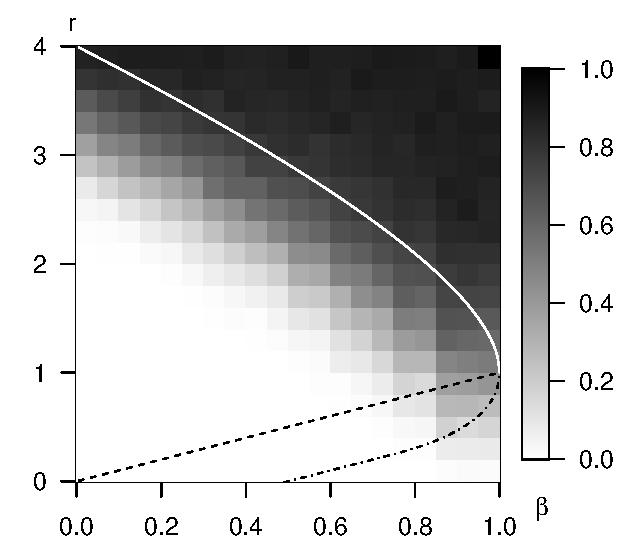
\includegraphics[width=0.4\textwidth]{./figures/simulated_phase_diagram_p100.eps}
      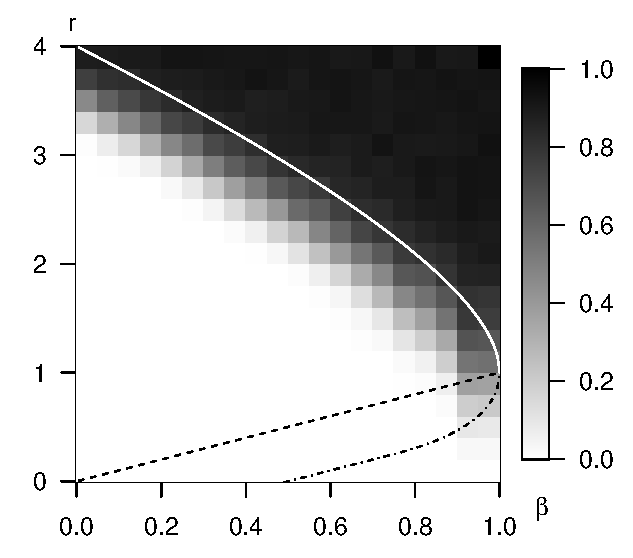
\includegraphics[width=0.4\textwidth]{./figures/simulated_phase_diagram_p10000.eps}
      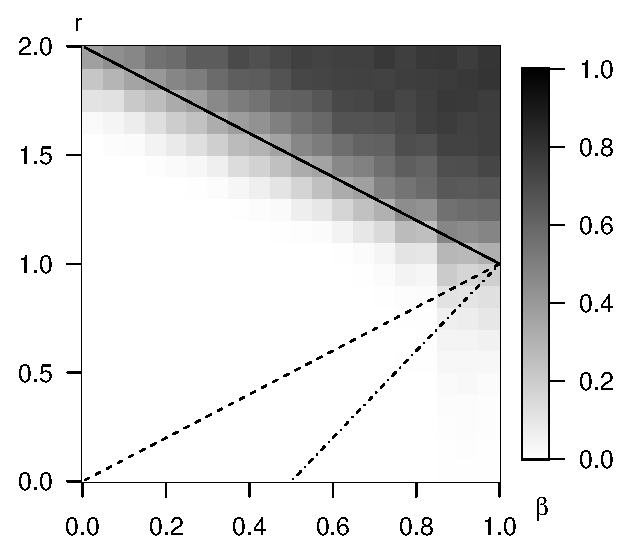
\includegraphics[width=0.4\textwidth]{./figures/simulated_phase_diagram_Laplace_p100_4.eps}
      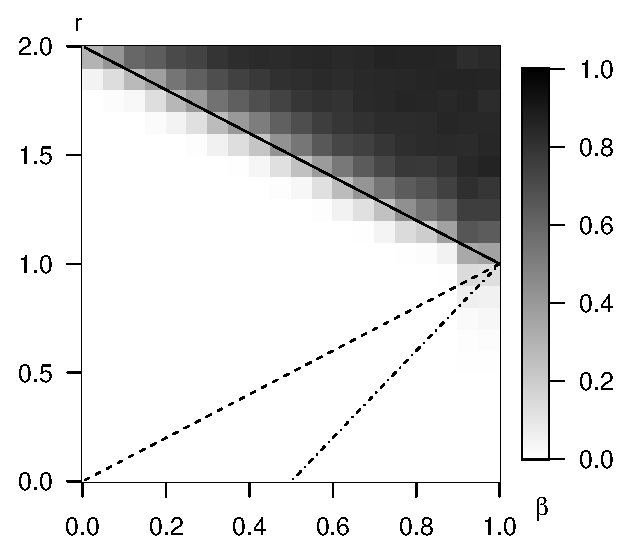
\includegraphics[width=0.4\textwidth]{./figures/simulated_phase_diagram_Laplace_p10000_4.eps}
      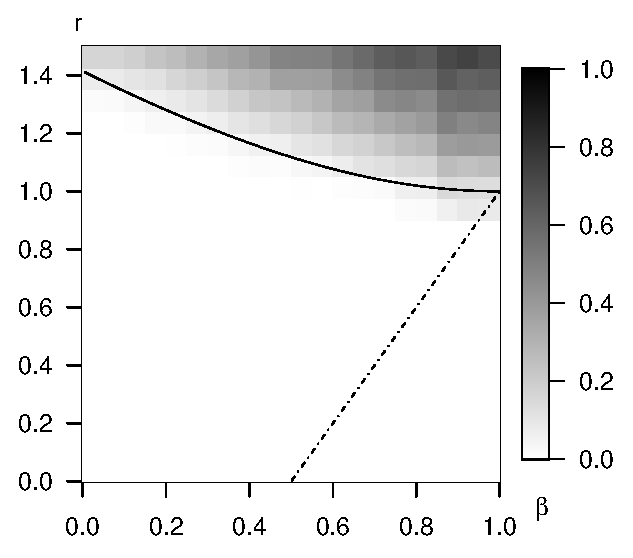
\includegraphics[width=0.4\textwidth]{./figures/simulated_phase_diagram_NLC_p100.eps}
      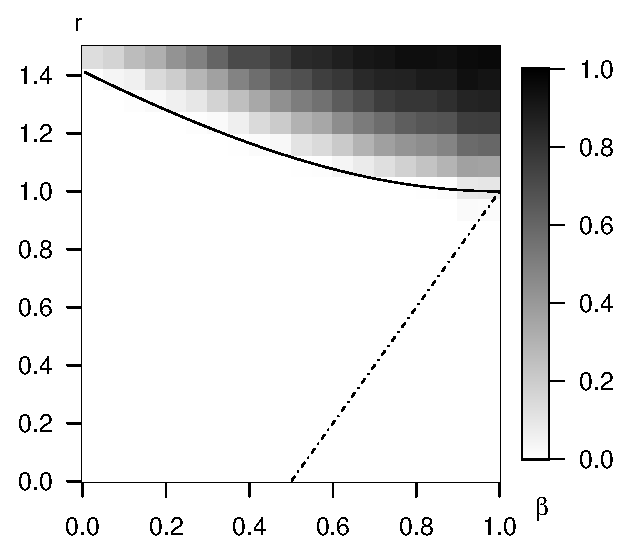
\includegraphics[width=0.4\textwidth]{./figures/simulated_phase_diagram_NLC_p10000.eps}
      \caption{The empirical probability of exact support recovery from numerical experiments, as a function of sparsity level $\beta$ and signal sizes $r$, 
      from Gaussian error models (upper panels), Laplace error models (middle panels), and generalized Gaussian with $\nu=1/2$ (lower panels); darker color indicates higher probability of exact support recovery. 
      The experiments were repeated 1000 times for each sparsity-signal size combination, and for dimensions $p=100$ (left panels) and $p=10000$ (right panels). 
      The numerical results agree with the boundaries described in Theorem \ref{thm:sufficient}. The convergence is noticeably slower for under the heavier 
      generalized Gaussian ($\nu=1/2$) errors.  For reference, the dashed and dash-dotted lines represent the weak classification and detection boundaries
       (see Chapter \ref{chap:phase-transitions}).
      \label{fig:phase-simulated}}
\end{figure}


